\documentclass[letterpaper,9pt,twocolumn,twoside,]{pinp}

%% Some pieces required from the pandoc template
\providecommand{\tightlist}{%
  \setlength{\itemsep}{0pt}\setlength{\parskip}{0pt}}

% Use the lineno option to display guide line numbers if required.
% Note that the use of elements such as single-column equations
% may affect the guide line number alignment.

\usepackage[T1]{fontenc}
\usepackage[utf8]{inputenc}

% pinp change: the geometry package layout settings need to be set here, not in pinp.cls
\geometry{layoutsize={0.95588\paperwidth,0.98864\paperheight},%
  layouthoffset=0.02206\paperwidth, layoutvoffset=0.00568\paperheight}

\definecolor{pinpblue}{HTML}{185FAF}  % imagecolorpicker on blue for new R logo
\definecolor{pnasbluetext}{RGB}{101,0,0} %



\title{\textcolor{black}{Data Analysis Report:} Root Insurance Co}

\author[a]{Issac Lee}

  \affil[a]{Department of Statistics \& Actuarial Science, 241 Schaeffer Hall, Iowa
City, Iowa 52242-1409}

\setcounter{secnumdepth}{0}

% Please give the surname of the lead author for the running footer
\leadauthor{Issac Lee}

% Keywords are not mandatory, but authors are strongly encouraged to provide them. If provided, please include two to five keywords, separated by the pipe symbol, e.g:
 

\begin{abstract}
This report illustrates how I approach the solution and make a decision
for Root insurance's data analysis project. The goal of this project is
to find the best-matched OBDII trip with a given trip data, which is
recorded by a customer's smartphone. In the first chapter, we learn how
to load the data set into the system. Next, we pick one sample trip from
each sensor and explore the data structure. Using these sample data, we
build a model and extend it to the whole data set in the later chapter.
Lastly, we illustrate the instructional manual for the written
\texttt{R} functions in the \texttt{Rootinsuarnce} package.
\end{abstract}

\dates{This version was compiled on \today} 

% initially we use doi so keep for backwards compatibility
% new name is doi_footer
\doifooter{\url{https://theissaclee.com}}

\pinpfootercontents{University of Iowa}

\begin{document}

% Optional adjustment to line up main text (after abstract) of first page with line numbers, when using both lineno and twocolumn options.
% You should only change this length when you've finalised the article contents.
\verticaladjustment{-2pt}

\maketitle
\thispagestyle{firststyle}
\ifthenelse{\boolean{shortarticle}}{\ifthenelse{\boolean{singlecolumn}}{\abscontentformatted}{\abscontent}}{}

% If your first paragraph (i.e. with the \dropcap) contains a list environment (quote, quotation, theorem, definition, enumerate, itemize...), the line after the list may have some extra indentation. If this is the case, add \parshape=0 to the end of the list environment.


\hypertarget{data-preparation}{%
\subsection{Data Preparation}\label{data-preparation}}

There are two telematics data set from independent sensors: GPS in a
smartphone, OBDII. The two data sets are stored in two separate files.
Here we assume that the two \texttt{JSON} files are extracted in the
working directory, which means you have the following two files in the
working directory:

\begin{quote}
mobile\_trips.json, obd2\_trips.json
\end{quote}

\hypertarget{data-load-and-structure}{%
\subsection{Data load and structure}\label{data-load-and-structure}}

Since the two files use the \texttt{JSON} format, we use the
\texttt{jsonlite} package to load the data.

\begin{Shaded}
\begin{Highlighting}[]
\KeywordTok{library}\NormalTok{(jsonlite)}

\CommentTok{# read mobile trip & obd2 trip}
\NormalTok{mobile_data <-}\StringTok{ }\KeywordTok{fromJSON}\NormalTok{(}\StringTok{"./mobile_trips.json"}\NormalTok{)}
\NormalTok{obd2_data <-}\StringTok{ }\KeywordTok{fromJSON}\NormalTok{(}\StringTok{"./obd2_trips.json"}\NormalTok{)}
\end{Highlighting}
\end{Shaded}

The smartphone data set consists of 44 trips, and the OBDII data set
consists of 41 trips. The column names of each data set and the data
types are as follows:

\begin{itemize}
\tightlist
\item
  OBDII data

  \begin{itemize}
  \tightlist
  \item
    trip\_id (\texttt{char}), timestamp (\texttt{dbl}), speed
    (\texttt{int})
  \end{itemize}
\item
  Mobile data

  \begin{itemize}
  \tightlist
  \item
    trip\_id (\texttt{char}), created\_at (\texttt{dbl}), timestamp
    (\texttt{dbl}), speed (\texttt{dbl}), accuracy (\texttt{int})
  \end{itemize}
\end{itemize}

Among these columns, we use only \texttt{timestamp} and \texttt{speed}
columns for the detecting algorithm.

\hypertarget{visualization-of-sample-trips}{%
\subsection{Visualization of sample
trips}\label{visualization-of-sample-trips}}

Fig \ref{fig:rawplot_obd2} shows the speed graph of a sample trip from
OBDII data. As we can see, the OBDII recorded the trip for about 1,200
seconds, and we do not know the unit of the vehicle speed. Fig
\ref{fig:rawplot_mobile} shows the speed graph of a sample trip from
mobile data. Note that the scale of the x-axis has been adjusted to
zero. By examing the data set, we can realize that the first trip from
each source corresponds to each other, as in Fig. \ref{fig:rawplot_obd2}
and Fig \ref{fig:rawplot_mobile}. The whole trip data from the
smartphone corresponds to the trip data from OBDII around 300 seconds.

\begin{figure}

{\centering 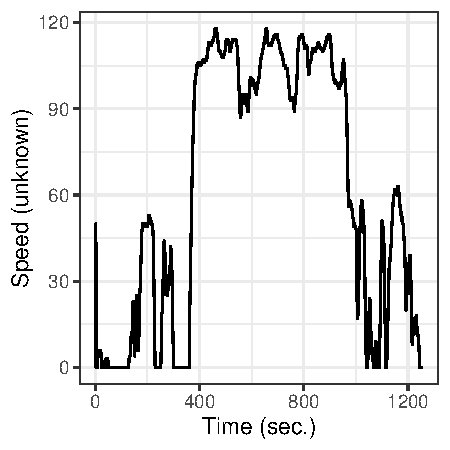
\includegraphics{report_issaclee_files/figure-latex/rawplot_obd2-1} 

}

\caption{A sample of speed graph of OBDII (the 1st trip).}\label{fig:rawplot_obd2}
\end{figure}

\begin{figure}

{\centering 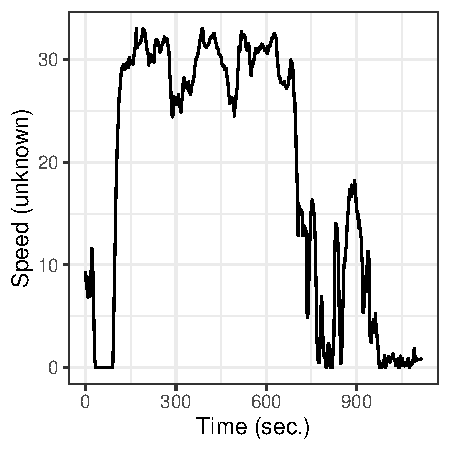
\includegraphics{report_issaclee_files/figure-latex/rawplot_mobile-1} 

}

\caption{A sample of speed graph of Smartphone (the 1st trip).}\label{fig:rawplot_mobile}
\end{figure}

\hypertarget{determine-the-conversion-factor-between-speed-scales}{%
\subsubsection{Determine the conversion factor between speed
scales}\label{determine-the-conversion-factor-between-speed-scales}}

Using this knowledge we found, we can figure out there is a conversion
factor between the two different speed scale from each source. If these
sensors recorded the same trip, their maximum speed of the trip should
be the same. Thus, we can calculate the conversion factor as follows:

\begin{Shaded}
\begin{Highlighting}[]
\CommentTok{# Conversion factor}
\KeywordTok{max}\NormalTok{(obd2_trip_sample1}\OperatorTok{$}\NormalTok{speed) }\OperatorTok{/}\StringTok{ }
\StringTok{  }\KeywordTok{max}\NormalTok{(mobile_trip_sample1}\OperatorTok{$}\NormalTok{speed)}
\end{Highlighting}
\end{Shaded}

\begin{ShadedResult}
\begin{verbatim}
#  [1] 3.570348
\end{verbatim}
\end{ShadedResult}

We can see that it is around 3.6. There are many units for speed, such
as miles per hour (mph), kilometers per hour (km/h), etc. Using the cue
that the smartphone sensor should use either \texttt{mph} or
\texttt{km/h,} we can easily guess that the OBDII uses \texttt{m/s}
since the relationship between \texttt{km/h} and \texttt{m/s} is as
follows:

\[
1 \ m/s = 3.6 \ km/h
\]

Thus, using the conversion factor and the lagging time (about 300 sec.),
we can guess our final output should be similar to Fig
\ref{fig:speedplot}. From now on, we use \texttt{km/h} as a speed scale
since the resulting plot re-confirms that the conversion factor is
right.

\begin{figure}

{\centering 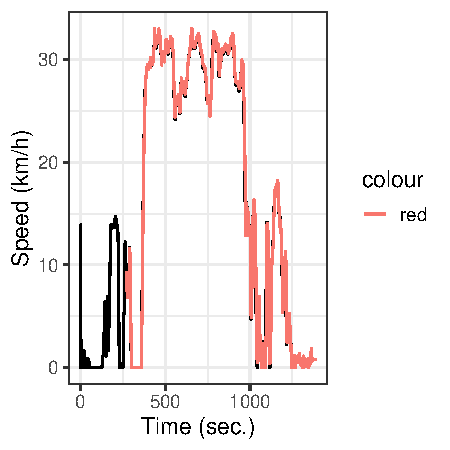
\includegraphics{report_issaclee_files/figure-latex/speedplot-1} 

}

\caption{A sample output of matched speed graph.}\label{fig:speedplot}
\end{figure}

\hypertarget{the-detection-algorithm-of-the-lagging-time}{%
\subsection{The detection algorithm of the lagging
time}\label{the-detection-algorithm-of-the-lagging-time}}

The next step is to automatically determine the lag time given that we
have two matched trips. We use the same sample trips used in the
previous section. In Fig. \ref{fig:speedplot}, the exact lag time for
smartphone trip data was 270 seconds. To detect the lagging time, we
need to consider every possible combination of these two trips by using
the sliding window algorithm.
\href{https://en.wikipedia.org/wiki/Convolution\#/media/File:Convolution_of_spiky_function_with_box2.gif}{This
Wikipedia web page} has an excellent visualization of the concept of the
algorithm. We consider the speed graph from OBDII as a fixed function
and the speed graph from a smartphone as a floating function in the
algorithm.

Let \(x \in \mathbb{R^{+}}\) be a real positive vector of size \(n_x\)
whose elements represent the speeds or a trip from a smartphone, while
\(y \in \mathbb{R^{+}}\) and \(n_y\) represents the speed and the size
of the speed vector from OBDII respectively.

\begin{equation*}
  \begin{aligned}
    x & = (x_1, x_2, ..., x_{n_x})^T \\
    y & = (y_1, y_2, ..., y_{n_y})^T
  \label{eqn:speedvector} 
  \end{aligned}
\end{equation*}

To implement the sliding window algorithm, we uses a dummy variable
\texttt{k} from 1 to \(n_x + n_y\) to search all the possible overlapped
combination of the two graph. For example, when \(k = 1\), we consider
the situation where \(x_{n_x}\) and \(y_1\) are overlapped each other.
When \(k=2\), \((x_{n_x - 1}, x_{n_x})\) and \((y_1, y_2)\) are
considered. Thus, for any \(k \leq n_x+n_y\) where \(k \in \mathbb{N}\),
the overlapped vectors, \(x^*\) and \(y^*\) can be written as follows;

\begin{equation}
  \begin{aligned}
  x^* &= (max(n_x - k, 1), ..., n_x - max(0, k - n_y))^T \\
  y^* &= (max(k-n_x, 1), ..., min(n_y, k))^T
  \label{eqn:slidingwindow} 
  \end{aligned}
\end{equation}

Equation \ref{eqn:slidingwindow} shows the compact expression for the
three cases:

\begin{itemize}
\tightlist
\item
  Case 1: \(k < n_x\) and \(k < n_y\)

  \begin{itemize}
  \tightlist
  \item
    \(x^* = (n_x - k, ..., n_x)\)
  \item
    \(y^* = (1, ..., k)\)
  \end{itemize}
\item
  Case 2: \(k > n_x\) and \(k < n_y\)

  \begin{itemize}
  \tightlist
  \item
    \(x^* = (1, ..., n_x)\)
  \item
    \(y^* = (k-n_x, ..., k)\)
  \end{itemize}
\item
  Case 3: \(k > n_x\) and \(k > n_y\)

  \begin{itemize}
  \tightlist
  \item
    \(x^* = (1, ..., n_y - (k-n_x))\)
  \item
    \(y^* = ((k-n_x), ..., n_y)\)
  \end{itemize}
\end{itemize}

\hypertarget{measure-for-the-similarity}{%
\subsection{Measure for the
similarity}\label{measure-for-the-similarity}}

There are many measures for the similarity of the two functions whose
domains are the same: area under the difference between the two
functions, the maximum difference of the two functions, etc. Among
these, we use the following measure for detecting the similarity between
the two-speed graphs:

\begin{equation}
  \begin{aligned}
 f(x, y) = \frac{\sqrt{\left(\sum_{i\in A}\left(x_{i}-y_{i}\right)^{2}\right)}}{|A|} + \frac{\lambda}{|A|}
  \label{eqn:sumofsquare} 
  \end{aligned}
\end{equation} where the vector \(x\) and \(y\) are the speed vector
from smartphone and OBDII, and the set \(A\) is the collection of the
pair of coordinates of OBDII and smartphone speed vectors overlapped
each other for fixed \(k\). Note that the function \(|.|\) indicates the
cardinality of a set. The reason for the division in Equation
\ref{eqn:sumofsquare} is to calculate the average of the errors.

Also, the penalty function, the second term in Equation
\ref{eqn:sumofsquare}, prevents the case where the dissimilarity of a
vector is so small since the length of the overlapped is too short. We
can put the weights on the penalty using \(\lambda\), and we use 10 for
\(\lambda\) value for this project. Since the value of \(f(x, y)\)
decreases when the two vectors, \(x\) and \(y\), are similar to each
other, the interpretation of the measure should be dissimilarity of the
two vectors. Fig. \ref{fig:laggedtime} shows the dissimilarity
concerning the \(k\) from 1 to 2354, which is the summation of the
length of the speed vectors. The index, which makes the dissimilarity to
be the smallest value, is \(k = 1374\). According to Equation
\ref{eqn:slidingwindow}, this corresponds to the 255th timestamp of the
OBDII trip.

\begin{figure}

{\centering 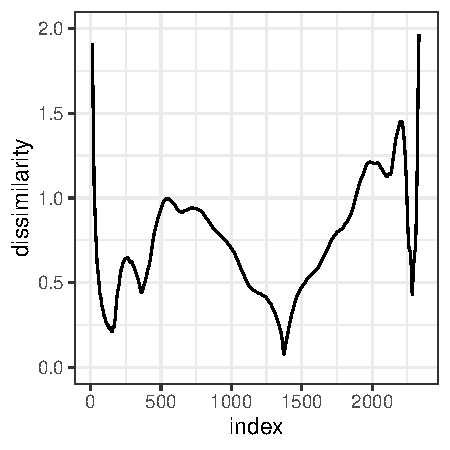
\includegraphics{report_issaclee_files/figure-latex/laggedtime-1} 

}

\caption{Dissimilarity measure for with respect to $k$. First trips from OBDII and smartphone.}\label{fig:laggedtime}
\end{figure}

\hypertarget{find-the-best-matched-trips}{%
\subsection{Find the best-matched
trips}\label{find-the-best-matched-trips}}

In the previous section, we have discussed how to find the lagging time
using dissimilarity measure. To find a best-matched OBDII trip for a
given smartphone trip, we find the OBDII trip whose minimum of the
dissimilarity with the given smartphone trip is the lowest among the
whole collection of OBDII trips in the data set. However, since we can
not guarantee that the lowest minimum of the dissimilarity implies that
the two trips matched each other, we set \(0.1\) as a threshold. Thus,
if the lowest minimum dissimilarity is less than 0.1, we conclude that
the pair of OBDII and smartphone trips matched with each other. Fig.
\ref{fig:dissimilarity} represents the minimum of dissimilarity for each
trip in OBDII data with the first trip in the mobile data set. The
dotted line, in Fig. \ref{fig:dissimilarity}, indicates the threshold
for the matched trip. Since the dissimilarity of the first trip is
lowest among OBDII trips and it is less than 0.1, we select that the
first trip in OBDII data as the best-matched trip with the first trip in
mobile data.

\begin{figure}

{\centering 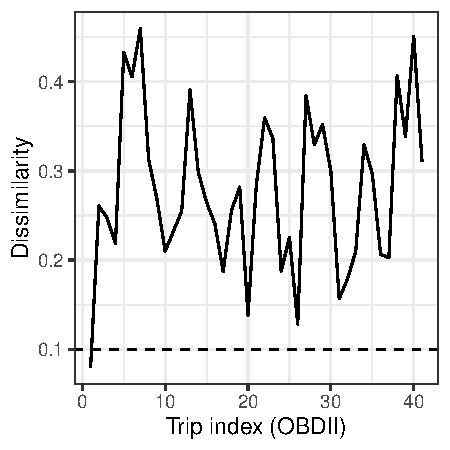
\includegraphics{report_issaclee_files/figure-latex/dissimilarity-1} 

}

\caption{Minimum values of dissimilarity for each trips in OBDII data set}\label{fig:dissimilarity}
\end{figure}

\hypertarget{user-manual}{%
\subsection{User manual}\label{user-manual}}

\hypertarget{installation}{%
\subsubsection{Installation}\label{installation}}

To install the \texttt{RootInsuarnce} package, save the
\texttt{RootInsurance\_0.1.0.tar.gz} file into your \texttt{R} working
directory, then run the following code.

\begin{Shaded}
\begin{Highlighting}[]
\KeywordTok{install.packages}\NormalTok{(}\StringTok{"./RootInsurance_0.1.0.tar.gz"}\NormalTok{,}
                 \DataTypeTok{repos =} \OtherTok{NULL}\NormalTok{, }\DataTypeTok{type =} \StringTok{"source"}\NormalTok{)}
\end{Highlighting}
\end{Shaded}

After the installation, you can load the package as follows:

\begin{Shaded}
\begin{Highlighting}[]
\KeywordTok{library}\NormalTok{(RootInsurance)}
\end{Highlighting}
\end{Shaded}

\hypertarget{load-telematics-data}{%
\subsubsection{Load telematics data}\label{load-telematics-data}}

Put your telematics file (JSON file format) in the working directory.
\texttt{LoadTelematics} function uses \texttt{jsonlite} package to load
the telematics trip using a list format in \texttt{R} as at the
beginning of this document.

\begin{Shaded}
\begin{Highlighting}[]
\CommentTok{# read mobile trip & obd2 trip}
\NormalTok{mobile_data <-}\StringTok{ }\KeywordTok{LoadTelematics}\NormalTok{(}\StringTok{"yourfile.json"}\NormalTok{)}
\NormalTok{obd2_data <-}\StringTok{ }\KeywordTok{LoadTelematics}\NormalTok{(}\StringTok{"yourfile.json"}\NormalTok{)}
\end{Highlighting}
\end{Shaded}

\hypertarget{find-the-best-obdii-trip-for-a-given-smartphone-trip}{%
\subsubsection{Find the best OBDII trip for a given smartphone
trip}\label{find-the-best-obdii-trip-for-a-given-smartphone-trip}}

The following \texttt{R} code selects the first smartphone trip in the
mobile data set as a target trip. Next, it finds the best-matched OBDII
trip using the \texttt{FindBestTrip} function and saves the result into
the \texttt{match\_info} variable.

\begin{Shaded}
\begin{Highlighting}[]
\CommentTok{# Select the second trip in the mobile data set}
\NormalTok{seleted_trip <-}\StringTok{ }\NormalTok{mobile_data[[}\DecValTok{1}\NormalTok{]]}

\CommentTok{# Find the best trip from OBDII data set}
\NormalTok{match_info <-}\StringTok{ }\KeywordTok{FindBestTrip}\NormalTok{(seleted_trip, obd2_data,}
                           \DataTypeTok{weight =} \OtherTok{TRUE}\NormalTok{)}
\end{Highlighting}
\end{Shaded}

The \texttt{match\_info} variable has the following seven information:

\begin{Shaded}
\begin{Highlighting}[]
\KeywordTok{summary}\NormalTok{(match_info)}
\end{Highlighting}
\end{Shaded}

\begin{ShadedResult}
\begin{verbatim}
#                  Length Class  Mode   
#  start_index_ref 1      -none- numeric
#  start_index_tar 1      -none- numeric
#  overlap_length  1      -none- numeric
#  dissimilarity   1      -none- numeric
#  macthed_trip    1      -none- numeric
\end{verbatim}
\end{ShadedResult}

\begin{Shaded}
\begin{Highlighting}[]
\NormalTok{match_info}
\end{Highlighting}
\end{Shaded}

\begin{ShadedResult}
\begin{verbatim}
#  $start_index_ref
#  [1] 256
#  
#  $start_index_tar
#  [1] 1
#  
#  $overlap_length
#  [1] 981
#  
#  $dissimilarity
#  [1] 0.07642238
#  
#  $macthed_trip
#  [1] 1
\end{verbatim}
\end{ShadedResult}

\hypertarget{visualization-of-the-matching-info.}{%
\subsubsection{Visualization of the matching
info.}\label{visualization-of-the-matching-info.}}

Once we find the best matching trip, you can visualize it using
\texttt{VisTrip} function as follows:

\begin{Shaded}
\begin{Highlighting}[]
\CommentTok{# Visualization}
\KeywordTok{VisTrip}\NormalTok{(seleted_trip, obd2_data, match_info)}
\end{Highlighting}
\end{Shaded}

\begin{center}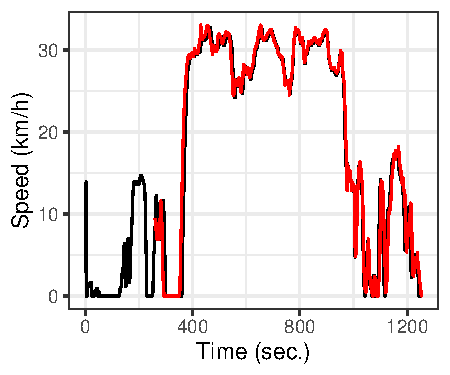
\includegraphics{report_issaclee_files/figure-latex/sampleresult-1} \end{center}

Note that if there is no best matching OBDII trip, this function shows a
possible candidate OBDII trip with a warning title.

\begin{Shaded}
\begin{Highlighting}[]
\CommentTok{# Select the second trip in the mobile data set}
\NormalTok{seleted_trip <-}\StringTok{ }\NormalTok{mobile_data[[}\DecValTok{39}\NormalTok{]]}

\CommentTok{# Find the best trip from OBDII data set}
\NormalTok{match_info <-}\StringTok{ }\KeywordTok{FindBestTrip}\NormalTok{(seleted_trip, obd2_data)}

\CommentTok{# Visualization}
\KeywordTok{VisTrip}\NormalTok{(seleted_trip, obd2_data, match_info)}
\end{Highlighting}
\end{Shaded}

\begin{center}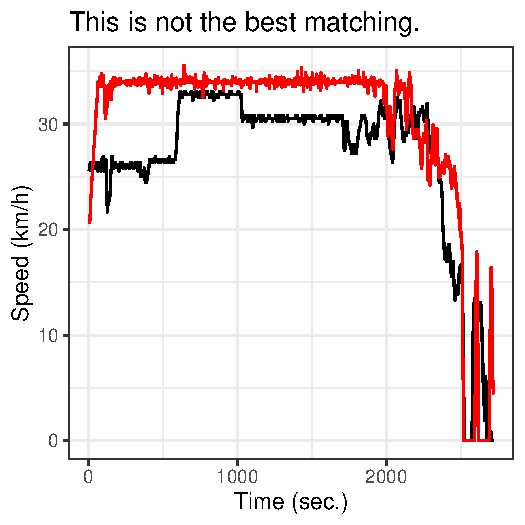
\includegraphics{report_issaclee_files/figure-latex/unnamed-chunk-9-1} \end{center}

%\showmatmethods


\bibliography{pinp.bib}
\bibliographystyle{jss}



\end{document}

